\documentclass[12pt]{article}
\usepackage[a4paper,margin=1in]{geometry}
\usepackage{tikz}
\usetikzlibrary{angles,quotes,calc}
\usepackage{amsmath}
\usepackage{hyperref}
\usepackage{graphicx}
\title{Understanding Circles}
\author{}
\date{}
\begin{document}
\maketitle
\tableofcontents

\section{What is a Circle?}
A circle is the set of all points that are the same distance from a fixed point called the \textbf{center}. The fixed distance is called the \textbf{radius}.

\begin{center}
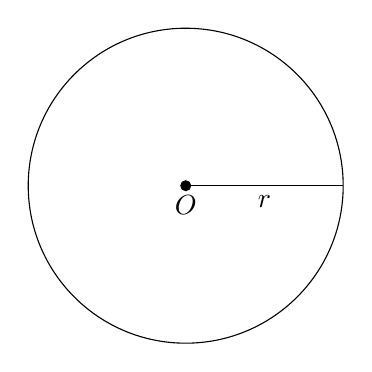
\begin{tikzpicture}[scale=1]
  \draw (0,0) circle(2cm);
  \fill (0,0) circle(2pt) node[below] {$O$};
  \draw (0,0) -- (2,0) node[midway, below] {$r$};
\end{tikzpicture}
\end{center}

\section{Important Parts of a Circle}
\subsection{Radius and Diameter}
The \textbf{radius} ($r$) is the distance from the center to any point on the circle. A \textbf{diameter} ($d$) is a line that passes through the center and touches the circle at two points. The diameter is twice the radius ($d = 2r$).

\begin{center}
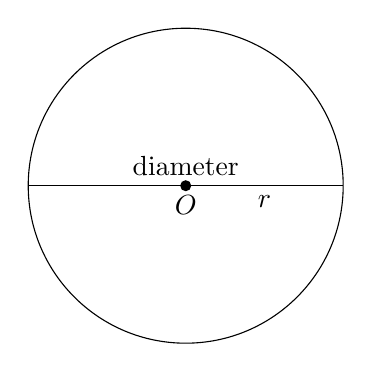
\begin{tikzpicture}[scale=1]
  \draw (0,0) circle(2cm);
  \fill (0,0) circle(2pt) node[below] {$O$};
  \draw (-2,0) -- (2,0) node[midway, above] {diameter};
  \draw (0,0) -- (2,0) node[midway, below] {$r$};
\end{tikzpicture}
\end{center}

\subsection{Chord and Arc}
A \textbf{chord} is a line connecting two points on the circle. An \textbf{arc} is the curved portion of the circle between those two points.

\begin{center}
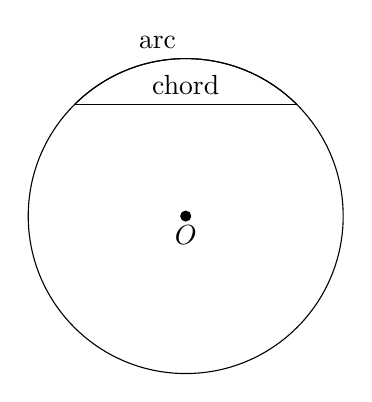
\begin{tikzpicture}[scale=1]
  \draw (0,0) circle(2cm);
  \fill (0,0) circle(2pt) node[below] {$O$};
  \coordinate (A) at (135:2cm);
  \coordinate (B) at (45:2cm);
  \draw (A) -- (B) node[midway, above] {chord};
  \draw (A) arc (135:45:2cm) node[midway, above left] {arc};
\end{tikzpicture}
\end{center}

\subsection{Sector and Segment}
A \textbf{sector} is a region enclosed by two radii and an arc. A \textbf{segment} is a region enclosed by a chord and an arc.

\begin{center}
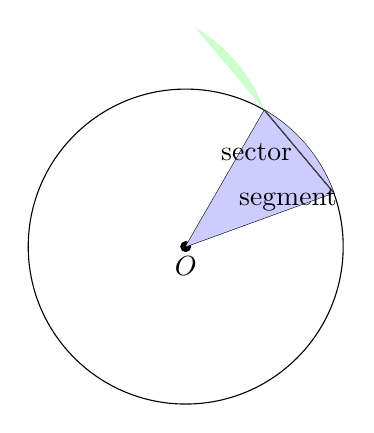
\begin{tikzpicture}[scale=1]
  \draw (0,0) circle(2cm);
  \fill (0,0) circle(2pt) node[below] {$O$};
  \coordinate (C) at (20:2cm);
  \coordinate (D) at (60:2cm);
  \draw (0,0) -- (C);
  \draw (0,0) -- (D);
  \fill[blue!20] (0,0) -- (C) arc (20:60:2cm) -- cycle;
  \draw (C) -- (D);
  \fill[green!20] (C) -- (D) arc (20:60:2cm) -- cycle;
  \node at (0.9,1.2) {sector};
  \node at (1.3,0.6) {segment};
\end{tikzpicture}
\end{center}

\subsection{Tangent}
A \textbf{tangent} is a line that touches the circle at exactly one point. The radius at the point of tangency is perpendicular to the tangent.

\begin{center}
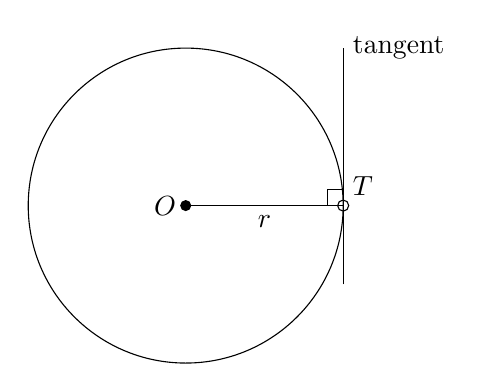
\begin{tikzpicture}[scale=1]
  \draw (0,0) circle(2cm);
  \fill (0,0) circle(2pt) node[left] {$O$};
  \draw (0,0) -- (2,0) node[midway, below] {$r$};
  \draw (2,-1) -- (2,2) node[right] {tangent};
  \draw (2,0) circle(2pt) node[above right] {$T$};
  \draw (1.8,0) -- (1.8,0.2) -- (2,0.2);
\end{tikzpicture}
\end{center}

\section{Perimeter and Area}
The perimeter of a circle is called its \textbf{circumference}. If the radius is $r$, then the circumference is
\begin{equation*}
C = 2\pi r.
\end{equation*}
The area enclosed by a circle is
\begin{equation*}
A = \pi r^2.
\end{equation*}

\section{Angle Facts}
\subsection{Central and Inscribed Angles}
A \textbf{central angle} has its vertex at the center. An \textbf{inscribed angle} has its vertex on the circle. The measure of an inscribed angle is half the measure of its intercepted arc.

\begin{center}
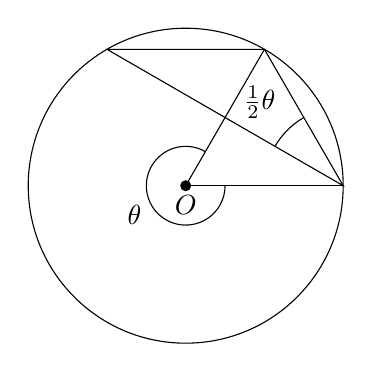
\begin{tikzpicture}[scale=1]
  \coordinate (O) at (0,0);
  \draw (O) circle(2cm);
  \fill (O) circle(2pt) node[below] {$O$};
  \coordinate (E) at (0:2cm);
  \coordinate (F) at (60:2cm);
  \coordinate (G) at (120:2cm);
  \draw (O) -- (E);
  \draw (O) -- (F);
  \draw (G) -- (E) -- (F) -- cycle;
  \pic [draw, "$\theta$", angle eccentricity=1.5] {angle = F--O--E};
  \pic [draw, "$\frac{1}{2}\theta$", angle eccentricity=1.5, angle radius=1cm] {angle = F--E--G};
\end{tikzpicture}
\end{center}

\subsection{Right Angle in a Semicircle}
Any angle formed by a diameter is a right angle.

\begin{center}
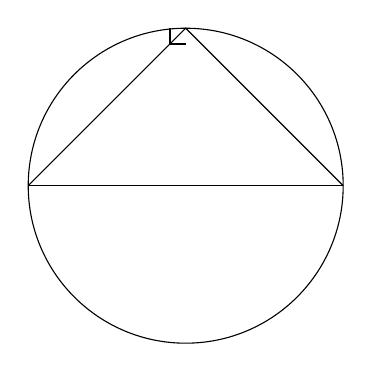
\begin{tikzpicture}[scale=1]
  \draw (0,0) circle(2cm);
  \coordinate (H) at (-2,0);
  \coordinate (I) at (2,0);
  \coordinate (J) at (0,2);
  \draw (H) -- (I);
  \draw (H) -- (J) -- (I);
  % right angle marker
  \draw (-0.2,2) -- (-0.2,1.8) -- (0,1.8);
\end{tikzpicture}
\end{center}

\section{Example}
\textbf{Problem:} A circle has radius $5\,\text{cm}$. Find its circumference and area.

\textbf{Solution:} Using $C = 2\pi r$ and $A = \pi r^2$,
\begin{align*}
C &= 2\pi (5) = 10\pi \approx 31.4\,\text{cm},\\
A &= \pi (5)^2 = 25\pi \approx 78.5\,\text{cm}^2.
\end{align*}

\section*{Summary}
\begin{itemize}
  \item A circle is defined by its center and radius.
  \item Important parts include radius, diameter, chord, arc, sector, segment, and tangent.
  \item Circumference $C = 2\pi r$ and area $A = \pi r^2$.
  \item Central angles equal their arc measure; inscribed angles are half their arc.
\end{itemize}

\end{document}
